\usetikzlibrary{arrows.meta,shapes.geometric}

\begin{frame}[fragile,label=pipeDeadlock]{pipe() deadlock}
\myemph{BROKEN} example:
\begin{lstlisting}[language=C++,style=small]
int child_to_parent_pipe[2], parent_to_child_pipe[2];
pipe(child_to_parent_pipe); pipe(parent_to_child_pipe);
if (fork() == 0) {
    /* child */
    write(child_to_parent_pipe[1], buffer, HUGE_SIZE);
    read(parent_to_child_pipe[0], buffer, HUGE_SIZE);
    exit(0);
} else {
    /* parent */
    write(parent_to_child_pipe[1], buffer, HUGE_SIZE);
    read(child_to_parent_pipe[0], buffer, HUGE_SIZE);
}
\end{lstlisting}
This will \myemph{hang forever} (if \texttt{HUGE\_SIZE} is big enough).
\end{frame}

\begin{frame}{deadlock waiting}
\begin{itemize}
\item child writing to pipe waiting for free buffer space
\item \ldots which will not be available until parent reads
\vspace{.5cm}
\item parent writing to pipe waiting for free buffer space
\item \ldots which will not be available until child reads
\end{itemize}
\end{frame}

\usetikzlibrary{arrows.meta,shapes.geometric}
\tikzset{
    >=Latex,
    resource/.style={draw,rectangle,very thick,align=center},
    resource m/.style={draw,rectangle,very thick,align=center,row sep=2mm},
    resource circle/.style={circle,fill=black,inner sep=0mm,minimum width=2.5mm},
    thread/.style={draw,ellipse,very thick,align=center},
    dependency/.style={draw,ultra thick,->},
    dependency future/.style={dependency,dotted},
    dependency reason/.style={align=center},
}

\begin{frame}{circular dependency}
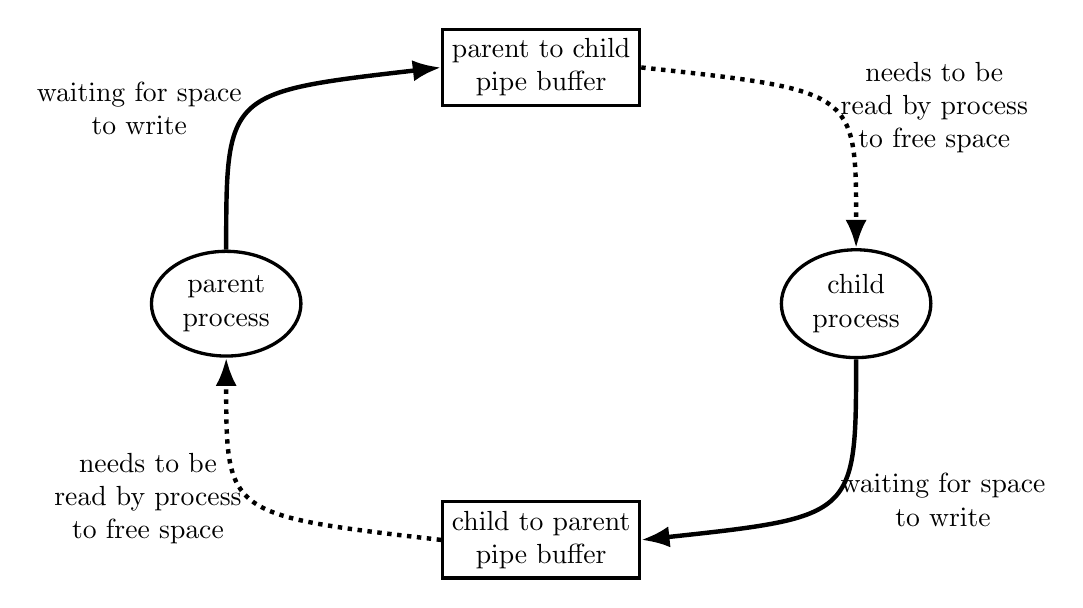
\begin{tikzpicture}
\node[resource] (parent to child) {
    parent to child \\ pipe buffer 
};
\node[resource] (child to parent) at ([yshift=-6cm]parent to child) {
    child to parent \\ pipe buffer 
};
\node[thread] (parent process) at ([xshift=-4cm,yshift=-3cm]parent to child) {
    parent \\ process
};
\node[thread] (child process) at ([xshift=4cm,yshift=-3cm]parent to child) {
    child \\ process
};

\path[dependency] (parent process.north) ..  controls ([yshift=2cm]parent process.north) .. (parent to child.west)
    node[midway,dependency reason,left] {
        waiting for space \\ to write
    };
\path[dependency] (child process.south) ..  controls ([yshift=-2cm]child process.south) .. (child to parent.east)
    node[midway,dependency reason,right] {
        waiting for space \\ to write
    };
\path[dependency future] (parent to child.east) .. controls ([yshift=2cm]child process.north) .. (child process.north)
    node[midway,dependency reason,right] {
        needs to be \\
        read by process \\
        to free space
    };
\path[dependency future] (child to parent.west) .. controls ([yshift=-2cm]parent process.south) .. (parent process.south)
    node[midway,dependency reason,left] {
        needs to be \\
        read by process \\
        to free space
    };
\end{tikzpicture}
\end{frame}
